\chapter{Static Computational Optical Undersampled Tracker}\label{chap:Scout}

\section{Motivation for the Static Computational Undersampled Tracker}

In large-area persistent surveillance, traditional \gls{isomorphic} sensing systems must acquire, process, store, and transmit large amounts of data to achieve high spatial and temporal resolution. These sensors are typically on airborne platforms or orbiting satellites which leads to a large \acrfull{swap-c}. However, if one is interested in estimating the location of moving objects (tracking) rather than reconstructing the entire object scene, the information content in the signal-of-interest is relatively low. One can significantly lower the \gls{swap-c} by using a task-specific approach. To address the challenges of traditional target tracking, several colleagues and I designed, built, and demonstrated such a device called the \acrfull{scout} \cite{townsend2012static, stenner2010static}. This chapter will provide details in to how we developed the \gls{scout}.

Most of the current experimental demonstrations of \gls{compressive imaging} try to reconstruct the entire object scene or spatial-temporal datacube. For example, the \gls{cacti} sensor uses a temporally varying psuedo-random coded aperture during a single \gls{fpa} exposure and attempts to reconstruct a spatial-temporal datacube \cite{llull2013coded}. In another experimental compressive imager, a rotating cylindrical lens measures scene data using an optical Radon transform and then reconstructs a static object scene \cite{evladov2012progressive}. While these architectures demonstrate the rapid progress that researchers have made towards compressive imaging, they emphasize reconstructing high dimensional data and require another post-processing step to extract task-specific information. Furthermore, this data will then need to be compressed again for storage or transmission. If one is concerned with only tasks, then reconstructing the entire scene as an intermediate step is unnecessary and even wasteful. 

Another example of \gls{compressive imaging} is the single pixel camera, discussed in \Cref{sec:multiplexingtocompressivesensing}. This sensor uses a \acrfull{dmd} to measure in any arbitrary basis, but must do so over many time-sequential measurements \cite{duarte2008single}. Each measurement is an integrated point-by-point multiplication of the scene locations with the \gls{dmd} array values. For temporally static scenes, this architecture allows an arbitrarily long exposure time (within the limit of detector saturation) to increase the \gls{snr} for each measurement. However, with temporally varying scenes it needs to record all the projections for each frame before the object moves.  Increasing the rate at which projections are made is possible, but this reduces exposure time and \gls{snr}. One way to overcome this is by implementing a parallel architecture of single pixel cameras, each with a different projection, see \Cref{fig:parallelcsimager2}. Clearly this will significantly increase the \gls{swap-c} of the architecture. Another issue with a fully parallel architecture, is that each camera will have a different entrance pupil location, producing parallax. One issue many computational sensor designs must deal with is ``over multiplexing''. All real optical \gls{adc} devices have a certain amount of dynamic range, in which linearity is valid. As the amount of light that is recorded increases, the amount of dynamic range being used fills up. Architectures which only use a single pixel are at greater risk for over multiplexing. 

\begin{figure}
	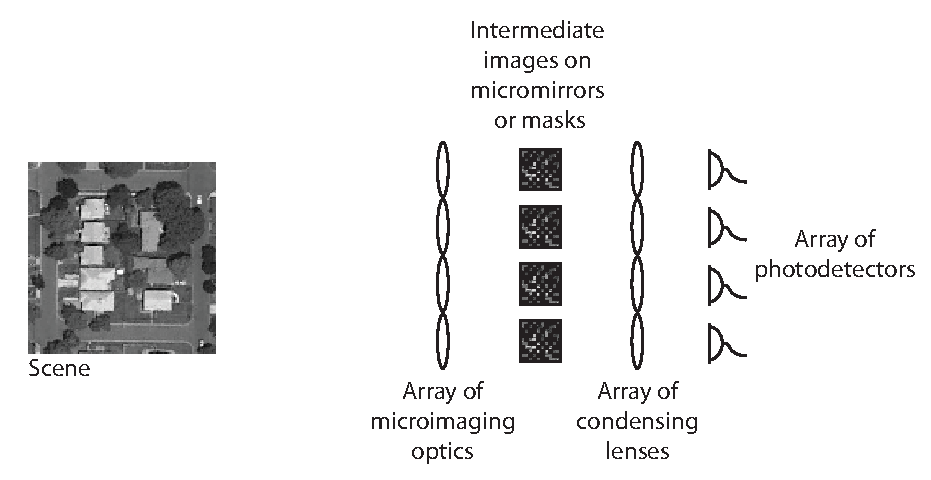
\includegraphics[scale=0.9]{parallelcsimager2}
	\captionof{figure}[The architecture of a hypothetical parallel single pixel camera to capture simultaneous projections.]{An example of a typical parallel optical CS architecture. Capturing $N_m$ simultaneous projections requires using $N_m$ spatial light modulators or masks and $N_m$ detector elements.}
	\label{fig:parallelcsimager2}
\end{figure}

A computational sensing architecture dedicated to target tracking rather than full object scene reconstruction, can significantly ameliorate these design trade-offs. We developed the \acrfull{scout} with the goal that measurements must be acquired ``single-shot'' using a conventional \gls{fpa} \cite{townsend2012static, poon2012advances}. The \gls{scout} system is an important step toward practical low-cost computational sensing for optical imaging. The system enables parallel ``single-shot'' acquisition of compressed, task-specific sensing oriented data, using a static (no moving parts) architecture. 

\begin{figure}
	\centering
	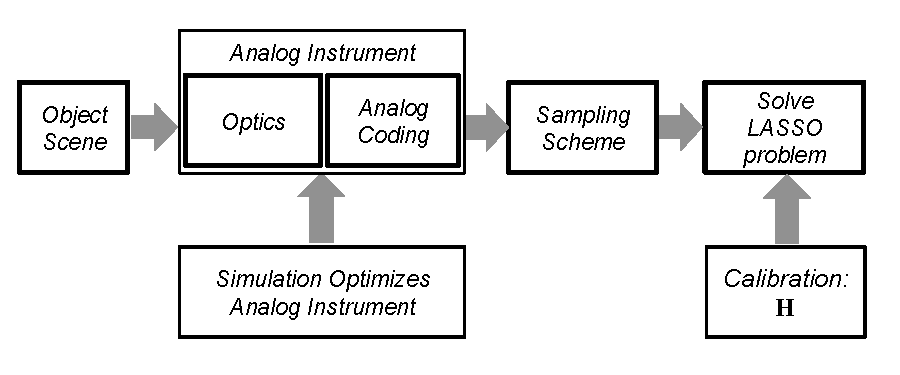
\includegraphics[scale=1.0]{scoutFlowchart}
	\captionof{figure}[Flowchart of \gls{scout} system architecture.]{A systems level flowchart of the \gls{scout} system. Light from the object scene propagates to the optical instrument which consists of a coded aperture (mask 1), an objective lens, and another coded aperture (mask 2), a \acrfull{fpa} then undersamples the coded object scene, measurement data is used to solve a \gls{lasso} problem. The parameters of the optical instrument is optimized using simulations to minimize the probability of tracking error. Calibration provides accurate measurement of the system matrix $\mb{H}$ to lasso optimization algorithm.}
	\label{fig:scoutFlowChart}
\end{figure}

A related static approach uses optical Radon projections \cite{kashter2012optical}. This instrument relies on a several cylindrical lenses to integrate the optical intensity from the object plane onto lines on the \gls{fpa}. The number of detector elements is much less than the native dimensionality of the object scene. For a single moving point in the field-of-view, two perpendicular Radon projections is enough to compute the change from frame to frame. However, the researchers found heuristically that four cylindrical lens are better for reconstructing the change information for an scene that included up to ten moving objects, called movers. 

A systems level flowchart of the \gls{scout} is shown in \Cref{fig:scoutFlowChart}. Like many computational sensors, it relies on the coding of the analog signal-of-interest prior to the \gls{adc} step and processes the measurement data using prior information and calibration data. The analog instrument was optimized using a custom ray-based simulation which evaluates a metric based on the simulated system matrix. In this chapter, I will discuss the \gls{scout} architecture in detail in \Cref{sec:ScoutArchitecture}, which uses a defocused imaging system with two binary amplitude masks. The \gls{fpa} samples at a much lower resolution than the native resolution of the object scene. While other compressive imaging systems have to reconstruct entire images, the \gls{scout} only reconstructs frame-to-frame differences. As a result the \gls{scout} requires significantly less bandwidth to transmit to a base station where the post-processing step can occur.


\section{SCOUT Architecture}\label{sec:ScoutArchitecture}

The goal of the \gls{scout} was to demonstrate a low \gls{swap-c} compressive target tracking sensor. The \gls{scout} architecture is designed to avoid the hardware scaling issues of the single-pixel camera. The trade-off for the ability to measure parallel projections is the loss of flexibility to implement arbitrary projections i.e. by using a \gls{slm}. However, rather than fully designing the projections themselves, I describe a process for optimizing the optical instrument  in \Cref{sec:ScoutSimulations}. Previous prototypes of the \gls{scout} architecture are described in \cite{stenner2010static, rivenson2010single}. 

The \gls{scout} system takes measurements that are both compressive and multiplexed: The number of measurements is less than the number of scene locations $N_m \ll N$, and each measurement must contain information about many scene locations. In this architecture, the number of measurements is the number of pixels in the \gls{fpa}. Intuitively this means that the system matrix must exhibit a many-to-few mapping from scene locations to \gls{fpa} elements. 


The \gls{scout} architecture is shown in \Cref{fig:scoutArchitecture}. In this architecture the \gls{multiplexing} occurs in the spatial domain by mapping multiple object scene locations to only a few detector pixels. To accomplish this, we created a structured blur. This blur allows the light from a single object point to be spread to several pixels on the \gls{fpa}. The most straightforward way to achieve a blur is by defocusing the image so that the \gls{psf} is broad, spanning many \gls{fpa} pixels. Since the number of \gls{fpa} pixels are less than the object scene resolution, the measurement is compressive. 


Like any aberration, defocus significantly reduces contrast of high spatial frequencies, so the measurements will be poorly conditioned for reconstruction. Therefore, we created high-frequency structure in the \gls{psf} by using two pseudo-random binary occlusion masks. Each mask is placed at different positions between the lens and the sensor. The separation between masks results in a spatially varying point-spread function. 




\begin{figure}
	\includegraphics[scale=1.2]{scoutArchitecture}
	\captionof{figure}[The SCOUT architecture.]{A diagram of the \gls{scout} architecture. A lens projects light through a pair of binary occlusion masks onto a low-resolution sensor which is defocused from the nominal image plane. This creates a spatially multiplexed shift-variant PSF incident on the \gls{fpa}.  }
	\label{fig:scoutArchitecture}
\end{figure}



As with many linear computational sensing architectures, the forward model is written in the form
%
\begin{equation}
	\mb{g} = \mb{H} \mb{f} + \mb{e}
\end{equation}
%
where $\mb{f}$ is the discrete representation of the object signal-of-interest, $\mb{g}$ is the measurement, $\mb{H}$ is the matrix which describes mapping of the object to the measurement, and $\mb{e}$ is the noise at each measurement. In this situation the signal-of-interest is actually the difference between two subsequent object scenes (frames) $\Delta \mb{f}$:
%
%
\begin{equation} 
\begin{split}
	\mb{g}_{k} &= \mb{H} \mb{f}_{k} + \mb{e}_{k} \\
	\mb{g}_{k+1} &= \mb{H} \mb{f}_{k+1} + \mb{e}_{k+1}
\end{split}
\end{equation}
%
Where the subscripts represent the $k^{th}$ readout from the \gls{fpa}.
%
\begin{equation}
	\Delta \mb{g} = \mb{g}_{k+1} - \mb{g}_{k} = \mb{H} \ap{ \mb{f}_{k+1} - \mb{f}_{k} } + \mb{e}_{k+1} - \mb{e}_{k} 
\end{equation}
%
%
so the forward model can be written as
%
\begin{equation}
	\Delta \mb{g} = \mb{H} \Delta \mb{f}  + \Delta \mb{e}
	\label{eq:scoutgHf}
\end{equation}
%
In this equation, the 2-dimensional difference frame and object scene have a resolution of $ R_x \times R_y$ elements, and are lexicography reordered into a $N \times 1$ column vector, $\Delta \mb{f}$ and $\mb{f}$. Similarly, the difference measurement and measurement $\Delta \mb{g}$ and $\mb{g}$ are $N_m \times 1$ vectors representing a 2-dimensional \gls{fpa} readout with a $ r_x \times r_y$ matrix which represents the low resolution measurement. The detector noise is represented by the $ N_m \times 1 $ vector $\mb{e}$. The system matrix $\mb{H}$ is thus an $N_m \times N $ matrix, where $N_m \ll N$ in order to the system to be considered compressive. The $n^{th}$ column of the matrix is the \gls{psf} of the $n^{th}$ location in the object scene. The resulting system matrix $\mb{H}$ demonstrates that the \gls{scout} is a spatially variant optical system and presents a block structure, as seen in the example shown in \Cref{fig:scoutSysResponse}.

\begin{sidewaysfigure}
	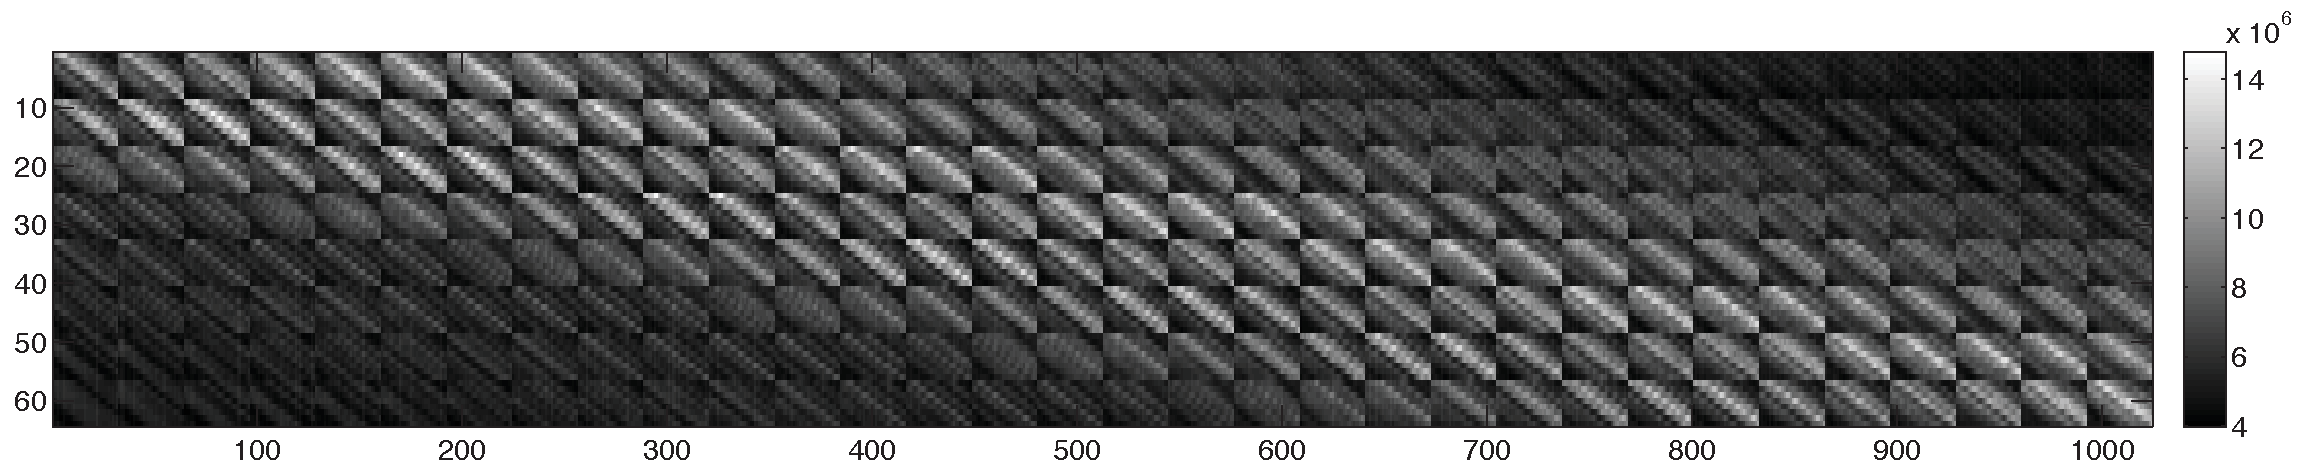
\includegraphics[scale=0.65]{scoutSysResponse}
	\captionof{figure}[An example of the system matrix of the \gls{scout}.]{An example of an experimentally measured of the system matrix of the \gls{scout} system. The approximate block-Toeplitz structure is clearly evident, as is the deviation from the Bernoulli or Gaussian ensembles typically considered in CS treatments. }
	\label{fig:scoutSysResponse}
\end{sidewaysfigure}


Referring back to the diagram of the \gls{scout} architecture shown in \Cref{fig:scoutArchitecture}. The object distance is much larger than the focal length of the lens so image of the scene occurs approximately one focal length from the lens $f_E$. The \gls{fpa} is placed some distance $d_{im}$ from the focal plane thus the total distance from the lens to the \gls{fpa} is $f_E + d_{im}$. Two binary occlusion masks, mask 1 and mask 2, are placed at distances $d_1$ and $d_2$ from the sensor. Mask 1 and 2 have associated fill factors $F_1$ and $F_2$ and pitch $p_1$ and $p_2$, respectively. 


\section{Optimizing the SCOUT}\label{sec:ScoutSimulations}

While the \gls{scout} lacks the ability to implement arbitrary measurement codes, we are able to adjust various physical parameters of the system such as defocus distance and mask fill factor to minimize reconstruction error. Adjusting each parameter in the actual prototype requires too much time, a more practical approach is to simulate the \gls{scout} architecture. In this section, I will discuss the simulation and define a metric that we used to evaluate different design parameters of the \gls{scout} without the need to reconstruct the difference frames. 

\subsection{Simulating a SCOUT System}

We developed a paraxial ray based simulation for the \gls{scout}. The simulation allows us to model the effects on the measurement as light travels through the lens and two masks and onto the detector plane. The lens is modeled as a single thin lens with transmittance function $t_f$ and the two masks have transmittance functions $t_1$ and $t_2$. From calibration measurements, the mask has a transmittances of $0$ where the mask is black and $0.88$ where the mask is clear. The lateral magnification of the scene and the two masks is calculated using similar triangles.

A simulated calibration occurs, in other words the simulation records the $r_x \times r_y$ PSF from each scene location in order to obtain the system matrix $\mb{H}$. Once $\mb{H}$ is known, we use it to simulate the low resolution measurements, $\mb{g}$, of the higher resolution scenes, $\mb{f}$. Subsequent simulated measurements are subtracted to find $\Delta \mb{g}$. We also did not add any noise. I have attached the simulation code in Appendix \ref{app:scoutSimCode}.


\subsection{Quantifying Reconstruction Error}

The \gls{mse} error metric is not suitable for our application because it weights all errors equally. For the task of motion tracking we classify errors into three types. A false positive occurs when the estimate shows an object where there is none. A false negative occurs when the estimate fails to show an object where one exists. As shift error occurs when an object is being tracked but appears in the wrong location. We developed a custom tracking error metric that weighs false negatives and false positives more than shift errors. This is because false negatives and false positives indicate a serious failure in the motion tracking task, while shift errors are less serious. We define tracking error as

\begin{equation}
	P = \frac{ | \mb{a}   \otimes \mb{\epsilon} |}{2N_{mv}}
	\label{eq:scoutErrorMetric}
\end{equation}
%
where
%
\begin{equation}
	\mb{a} = 
	\begin{bmatrix}
	    1/9 & 1/9 & 1/9 \\
	    1/9 & 1/9 & 1/9 \\
	    1/9 & 1/9 & 1/9 
	\end{bmatrix}
\end{equation}
%
where the error $\mb{\epsilon}$ is the difference between the true and reconstructed difference frames
%

\begin{equation}
	\mb{\epsilon} = \Delta \mb{f} - \Delta \mbh{f}
\end{equation}
%
and $N_{\text{mv}}$ is the number of movers in the scene. To reduce the penalty for one-pixel shift errors, the error frame is convolved with a three pixel averaging kernel $\mb{a}$. The absolute value is taken in order to count positive and negative errors equally, and the error is divided by $2N_{mv}$ to make the metric independent of the number of movers. 

\subsection{Optimizing Optical System Parameters}

Now that I have explained the simulation and the custom error metric for tracking, I can finally begin to discuss how we optimized some of the parameters to reduce the reconstruction error. Both the simulation and experimental study demonstrates a relationship between mask position and pitch: the tracking error is very sensitive to the \emph{projected} mask pitch on the \gls{fpa}. Furthermore, increasing the mask seperation reduced tracking error, generating a highly space-variant \gls{psf}. With these observations in mind, we focus our study on the mask pitches ($p_1$, $p_2$) as well as the defocus distance $d_{im}$. 

A brute force search, using the \gls{lasso} solver at each step is computationally intensive. We wanted a simple to compute metric which can predict tracking error. So we developed a custom metric inspired by the coherence parameter from the compressive sensing community, see \Cref{eq:coherenceDef1}. We created a customized coherence parameter $\mu$, 
%
\begin{equation}\label{defofcoherence}
    \mu = \max{\left| \langle h_i, h_j \rangle \right|} ;  \qquad i \neq j
\end{equation}
%
which is the maximum absolute value of the inner product between unique columns $h_i$ and $h_j$ of $\mb{H}$. The columns are unnormalized because their relative magnitude is related to the physical light throughput. 

Notice that although system matrices with nearly pairwise orthogonal columns will result in small coherence values, system matrices with numerically small entries can accomplish the same. Optimizing $\mb{H}$ for minimum coherence would drive total system throughput down. To eliminate this effect we normalized $\mb{H}$:

\begin{equation}
	\mb{H}_{norm} = \frac{ \mb{H} }{ \sum_{m = 1}^{N_m} \sum_{n = 1}^{N} h_{m,n} }
\end{equation}
%
where $N_m$ and $N$ are the total number of rows and columns in the system matrix. Physically, this normalization represents division by the sum of each PSF’s light throughput. The coherence of a system matrix normalized in this way cannot be biased by reducing throughput. One consequence of this normalization is that mask fill factor cannot be optimized.

\begin{figure}[!ht]
	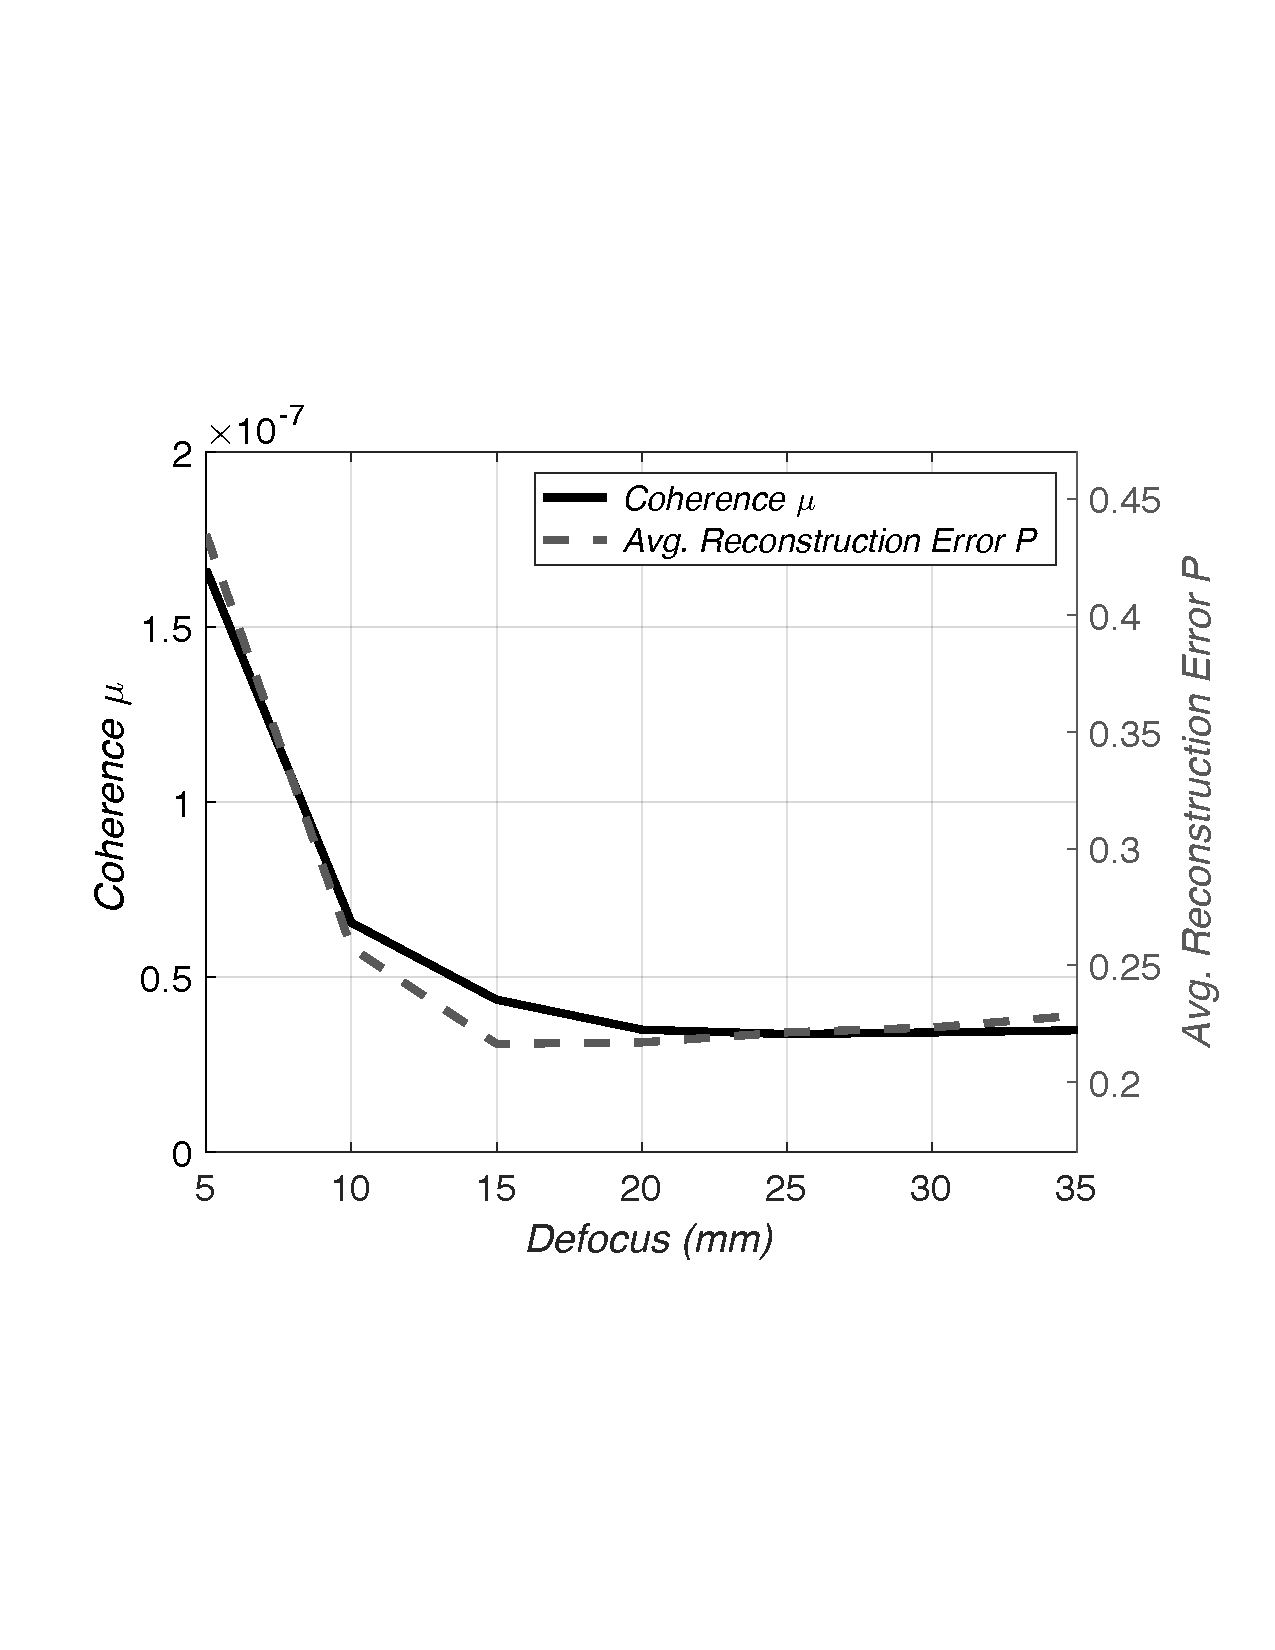
\includegraphics[scale=0.75]{coherenceAndReconErrorVsDefocus}
	\captionof{figure}[The coherence and reconstruction error versus defocus distance.]{The coherence $\mu$ (left vertical axis - black) and reconstruction error P (right vertical axis - dashed gray) plotted as a function of defocus distance $d_im$. }
	\label{fig:coherenceAndReconErrorVsDefocus}
\end{figure}

\begin{figure}[!ht]
	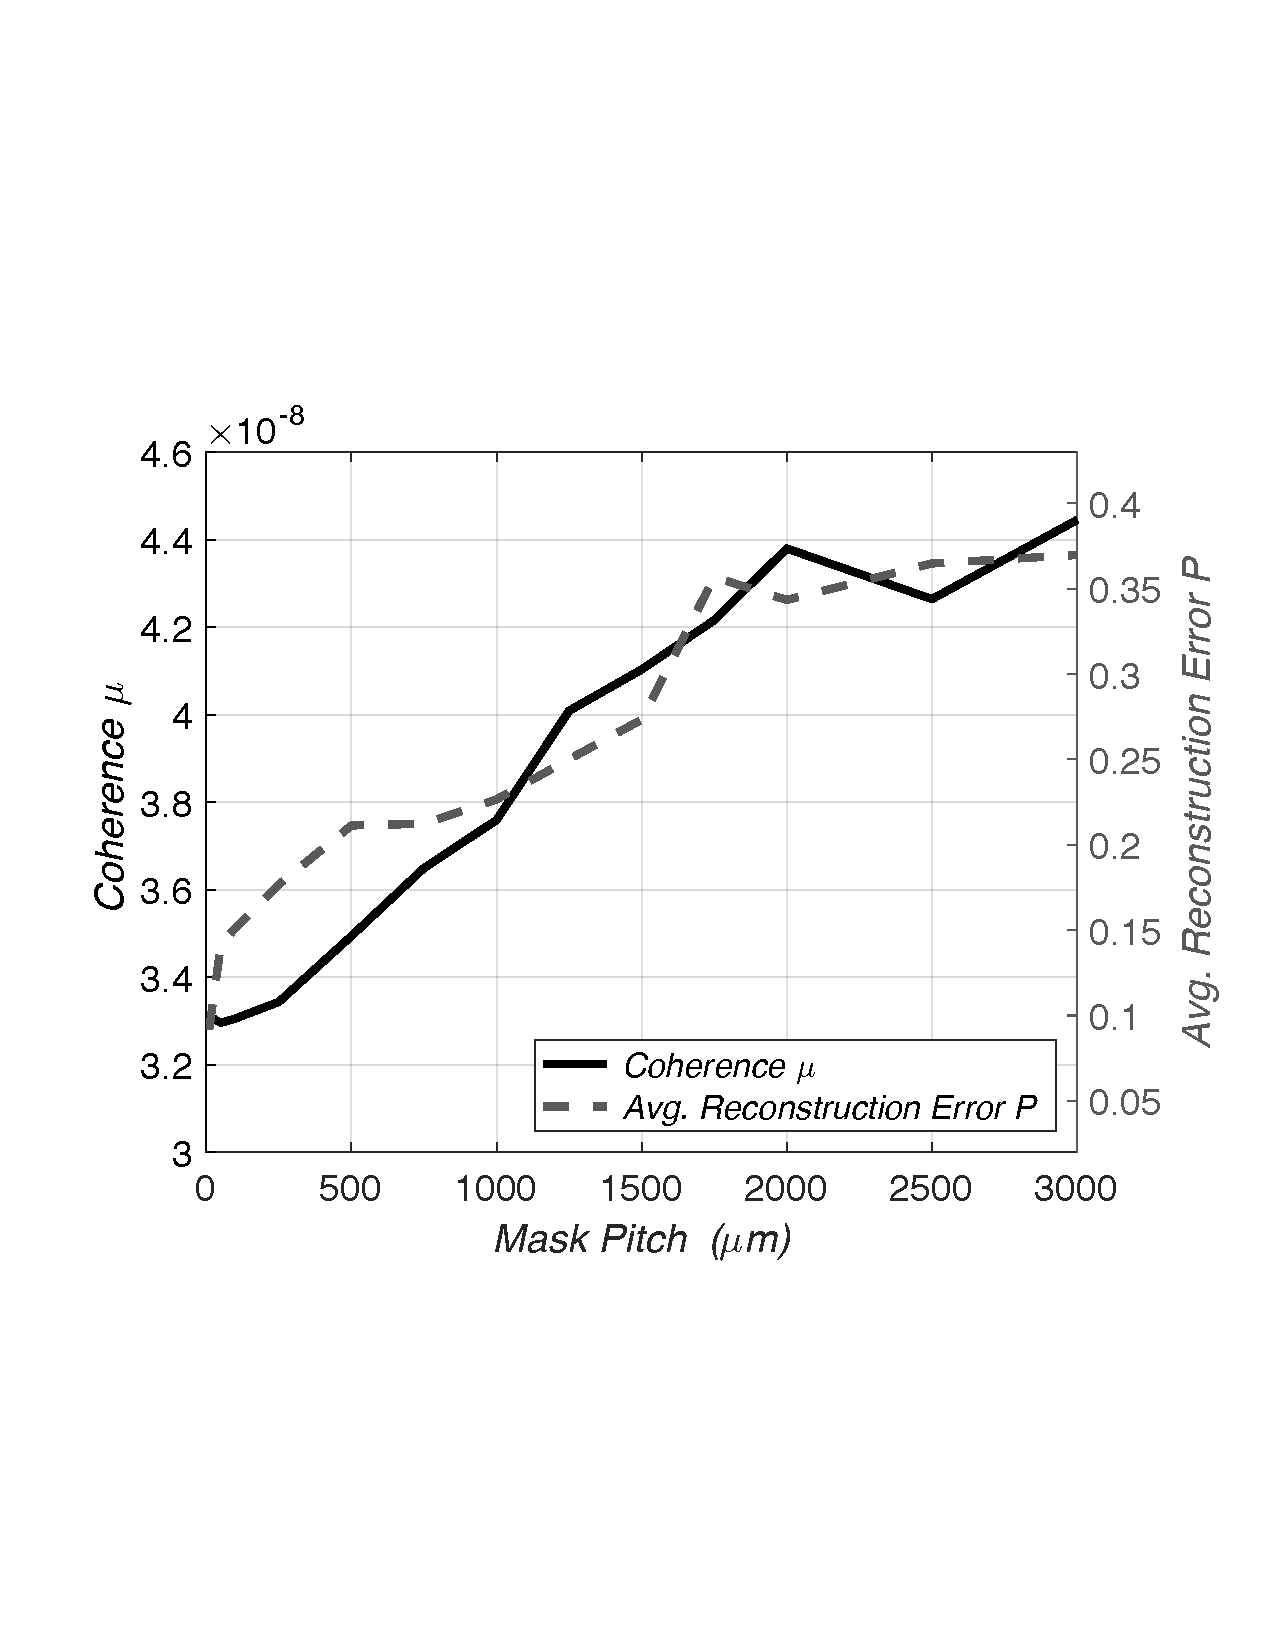
\includegraphics[scale=0.75]{coherenceAndReconErrorVsMaskPitch}
	\captionof{figure}[The coherence and reconstruction error versus pitch of mask 2.]{The coherence $\mu$ (left vertical axis - black) and the reconstruction error P (right vertical axis - dashed gray) is plotted as a function of the pitch of mask 2 }
	\label{fig:coherenceAndReconErrorVsMaskPitch}
\end{figure}


\begin{figure}[!ht]
	\centering
	\includegraphics[scale=0.65]{scoutExpSetup1}
	\captionof{figure}[Photograph of \gls{scout} recording a moving object scene of a black background.]{The camera captures images of scenes displayed on a plasma television approximately 2 meters away..}
	\label{fig:scoutExpSetup1}
\end{figure}

\begin{figure}[!ht]
	\centering
	\includegraphics[scale=0.85]{scoutExpSetup3}
	\captionof{figure}[Photograph of \gls{scout} camera disassembled to show the lens and the first mask.]{The camera disassembled to show the camera body, the optical tube and the custom fabricated lens holder which goes inside the lens tube.}
	\label{fig:scoutExpSetup3}
\end{figure}

To demonstrate the effectiveness of the modified coherence parameter as a predictor of reconstruction error trends, I ran several simulations with complete reconstructions in order to compare reconstruction error to coherence. \Cref{fig:coherenceAndReconErrorVsDefocus} shows that reconstruction error and the coherence parameter follow similar trends for different defocus distances when all other parameters are held constant. \Cref{fig:coherenceAndReconErrorVsMaskPitch} shows similar agreement when varying values of mask pitch $p_2$.

The simulations demonstrate the viability of the architecture and provide an efficient way to optimize most architecture parameter values using the simulated system matrix coherence. Mask throughput cannot currently be optimized because the custom coherence metric is normalized by full system throughput. The problem of finding optimal mask throughput warrants further investigation.

\section{Experiment}\label{sec:ScoutExperimentalResults}

\subsection{Experimental Setup}

For the experiment, the captured image resolution $r_x \times r_y$ is $8 \times 8$, while the ground-truth and reconstructed frame differences have a resolution $R_x \times R_y$ of $32 \times 32$. To simulate a low-resolution detector, the camera captures the scenes at $128 \times 128$ sensor pixels and the images are binned down to $8 \times 8$ before being used in reconstruction. 


We used a SBIG Model ST-7XMEI CCD camera with modified optics. The object scenes were displayed on a plasma television monitor. Figures \ref{fig:scoutExpSetup1} and \ref{fig:scoutExpSetup3} shows a photograph of the experimental setup. The optical system of the camera includes a 35 mm focal length lens and two random amplitude binary masks. Each mask was printed on transparencies using a high resolution laser printer. Mask 1 has pitch $p_1 = 30$ microns and fill factor $F_1 = 0.4$ and is located at a distance $d_{m1} = 14mm$ from the sensor. Mask 2 has pitch $p_2 = 500$ microns and fill factor $F_2 = 0.2$ and is located at a distance $d_{m2} = 57mm$ from the sensor. These parameters were chosen based on the aforementioned optimization process. A plasma monitor was used because it provides a higher contrast compared to the traditional liquid crystal displays (LCD). However, the black background of the plasma monitor still produced a small amount of irradiance, which is a source of systematic error and potentially reduces the usable amount of dynamic range. 
\subsection{Calibration}\label{ssec:ScoutCalibration}

Instruments based on compressive sensing rely heavily on accurate calibration. Especially important is the knowledge of the system matrix $\mb{H}$ to prevent reconstruction or task-specific sensing errors. The \gls{scout} architecture is no different. Inaccurate calibration dramatically affects the tracking error.  Furthermore, because of the non-isomorphic nature of compressive sensing, it is difficult to look at the system matrix and intuitively tell whether it will lead to good results. In this section, I will describe the calibration procedure for the \gls{scout} architecture. 

Conceptually the calibration procedure is a straightforward. The goal is to experimentally determine the system matrix $\mb{H}$. Each column of the matrix   is the \acrfull{psf} due to a ``point'' at the $n^{th}$ location in the object scene. All one needs to do is display the point at each location and store the measurement in the respective column of $\mb{H}$. 


There are several practical issues in the calibration process for the \gls{scout}. Calibration itself is a measurement process, noise is present in each measurement. To mitigate the effects of noise, we cooled the \gls{ccd} in the camera to $0$ degrees Celsius using the built-in thermoelectric cooling (TEC). We also increased the exposure time to 1.0 seconds. While it is possible to continue increasing the exposure time, we found that increasing the exposure time past this did not significantly reduce the tracking error metric.

To eliminate any systematic error due to light pollution, we constructed a light-tight box using 80/20 aluminum framing, black poster board, and black gaffer tape. This box enclosed the entire \gls{scout} and the plasma monitor. We also found that the plasma monitor emitted a certain amount of light even though it is set to zero. To mitigate this, we take several dark frame measurements, which is a measurement with the plasma monitor set to all zero and then averaged. This averaged dark frame measurement is subtracted from each \gls{psf} measurement. 

Another issue with the plamsa is that the intensity varies after a few minutes. Therefore, every 60 seconds we pause the calibration procedure and set the entire screen to all white. This resets the intensity levels and a new set of dark frame measurements is recorded. The calibration sequence is then allowed to continue. 

Another issue with the plamsa monitor is that when a particular pixel is illuminated, the intensity of the adjacent pixels change. So when the next pixel is illuminated, that intensity is different compared to the intensity we measure if the adjacent pixel had not been turned on. In other words, turning on pixel $n$ changes the intensity at pixel $n+1$ when it is turned on. In order to mitigate this effect, we created a psuedo-random sequence so that after a certain amount of time, the effect of a neighboring pixels activity is reduced. The total time to calibrate the \gls{scout} is approximately 20 minutes. 

Remember that an isomorphic sensor is represented by the identity matrix. In comparison, in the \gls{scout}, the spatially varying blurred \gls{psf} leads to an approximate block-Toeplitz structure for the system matrix, with approximate Toeplitz structure within individual blocks due to the shifting \gls{psf}. This circulant structure is modified by random variations corresponding to the differing projections created by the two masks. Psuedo-case describing the calibration is given in Appendix \ref{app:scoutPsuedoCode}.  




\subsection{Reconstruction: $\ell_1$ regularized Least Squares Minimization}

Given $\Delta \mb{g}$ and $ \mb{H} $, reconstructing the difference frame $\Delta \mb{f}$, is a highly underdetermined problem given no other prior knowledge. As discussed in \Cref{sec:compressiveSesing}, several important theoretical results show that it is possible to accurately recover $\Delta \mb{f}$ if the sparsity $K$ is low relative to the number of measurements $N_m$ and the \gls{rip} is satisfied. Inspired by these results, we turn to algorithms designed to solve the $\ell_1$ regularized \gls{ls} (\gls{lasso}) problem:
%
\begin{equation}
	\Delta \mbh{f} = \argminA_{\Delta \mb{f}} \: \| \mb{H} \Delta \mb{f} - \Delta \mb{g} \|_{2}^{2} + \tau \| \Delta \mb{f} \|_1
	\label{eq:scoutl1regls}
\end{equation}
%
Given $\Delta \mb{g}$ and $ \mb{H} $, the reconstruction algorithm finds a solution $\Delta \mbh{f}$ that minimizes this objective function. 


We used the \texttt{l1\_ls} toolbox for MATLAB which implements an optimization technique based on Interior-Point methods \cite{kim2007interior}. The \texttt{l1\_ls} function requires several input arguments: $\Delta \mb{g}$, $ \mb{H} $, $\tau$ the regularization parameter, and a parameter called the relative tolerance, \texttt{rel\_tol}. As I discussed in \Cref{sec:compressiveSesing}, $\tau$ is a tuning parameter that is used to tell the optimization algorithm how much to weight the sparsity of the solution. Large $\tau$ tend to drive the solutions towards lower values of sparsity, \gls{sparseSym}. The \texttt{rel\_tol} controls how well the solution should agree with the data. Low values of \texttt{rel\_tol} tend to force the \texttt{l1\_ls} to run many iterations until the a threshold has been reached. While large values of \texttt{rel\_tol} tend to produce poorer reconstruction results but less optimization iterations. 

We found that a regularization parameter of $\tau= \left( 1 \times 10^{-9} \right) \| 2 \: \mb{H}_{cal}^T \: \Delta \mb{g} \|_{\infty}$ works well for experimental reconstruction. Where $\mb{H}_{cal}$
is the system matrix measured from calibration and $\| \cdot \|_{\infty}$ is the infinity norm. The \texttt{rel\_tol} is set to $1 \times 10^{-4}$.

Finding the correct regularization parameter is one of the major issues for many algorithms designed for compressive sensing. In our experiment, we had to run the reconstruction over many iterations with varying $\tau$ in order to find the appropriate value. Unfortunately this also depends on the sparsity of the signal-of-interest. Therefore, large numbers of movers may have a different optimal value for $\tau$. The value of $\tau$, we reported works well from one to ten movers in our experiment.

\subsection{Experimental Results}
Experimental results for a ten difference frame sequence is shown in Appendix \ref{app:scoutExpResults}. The object scenes contains two dots (movers) changing position on a black background. Difference frame 1 of this sequence is shown in \Cref{fig:scout_fig10_un}. The top row shows two consecutive, before and after, $\mb{f}_1$ and $\mb{f}_2$, frames of the scene and the ground-truth difference frame $\Delta \mb{f}$, all at $32 \times 32$ resolution. The bottom row shows the difference of corresponding $8 \times 8$ measurement frames, $\Delta \mb{g}$. Finally, the $32 \times 32$ reconstructed difference frame is shown at the bottom right, $\Delta \mbh{f}$. 

Initially, the amplitude of the movers in the estimated difference frame to did not agree qualitatively with the amplitude of the ground truth difference frame. We realized that this was due to the fact that the exposure time during calibration was not the same as the exposure time during the actual experiment. By normalizing the system matrix obtained during calibration by the ratio of exposure times, we were able to demonstrate quantitative agreement with the ground-truth:

\begin{equation}
	\mb{H}_{recon} = \frac{t_{exp}}{t_{cal}} \mb{H}_{cal}
	\label{eq:ScoutCalibrationMatrixScaling}
\end{equation}
%
where $t_{exp}$ and $t_{cal}$ are the experiment and calibration exposure times, respectively. This scaling accounts for the physical effect of increased photon collection (and hence photodetector counts) as a function of increased exposure time. The resulting peaks are easily identified against background noise.

\begin{figure}
	\centering
	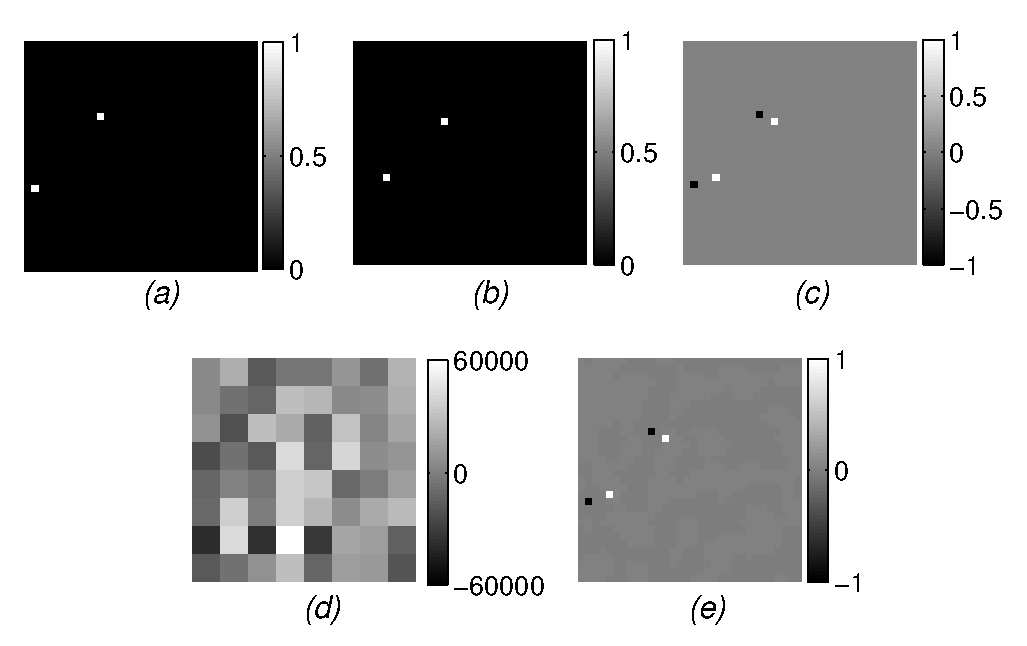
\includegraphics[scale=0.75]{scout_fig10_v2.eps}
	\captionof{figure}[Difference frame 1 of a sequence of two movers on a black background.]{A reconstruction of a $32 \times 32$ scene with two movers of equal amplitude on a black background. (a) ground-truth scene 1 (b) ground-truth scene 2 (c) ground-truth frame difference and (d) measured $8 \times 8$ frame difference, scaled so that it is discernible (e) reconstructed $32 \times 32$ difference frame}
	\label{fig:scout_fig10_un}
\end{figure}

\begin{figure}
	\centering
	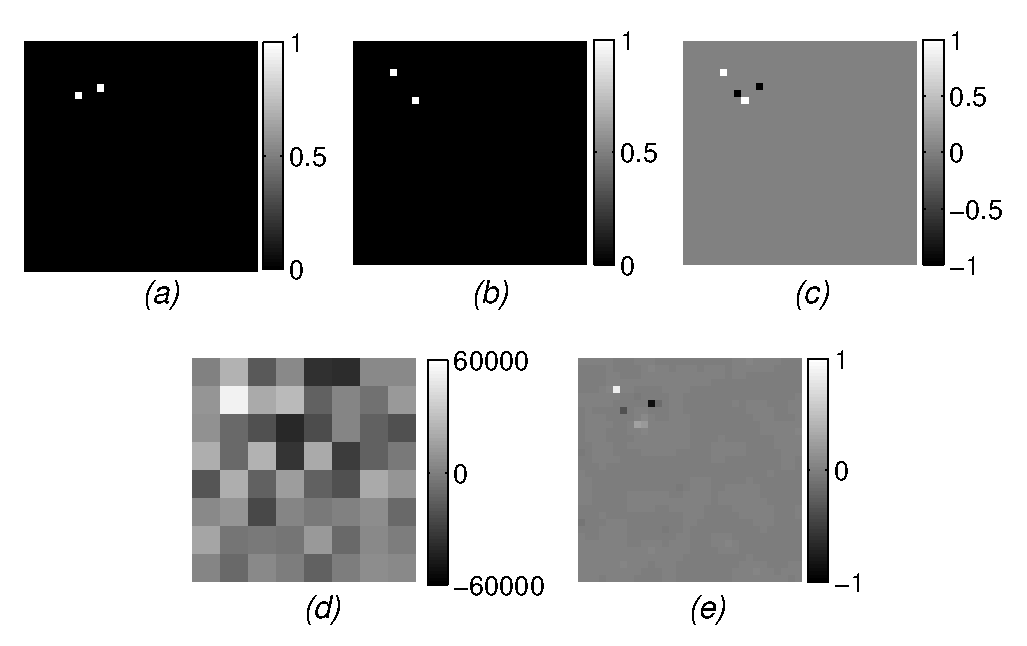
\includegraphics[scale=0.75]{scout_fig11_v2.eps}
	\captionof{figure}[Difference frame 9 of a sequence of two movers on a black background.]{A reconstruction of $32 \times 32$ scene with two movers of equal amplitude on a black background. This frame shows the results when the past and present mover locations are adjacent in the difference frame. (a) ground-truth scene 1 (b) ground-truth scene 2 (c) ground-truth frame difference and (d) measured $8 \times 8$ frame difference, scaled so that it is discernible (e) reconstructed $32 \times 32$ difference frame}
	\label{fig:scout_fig11_un}
\end{figure}


\begin{figure}
	\centering
	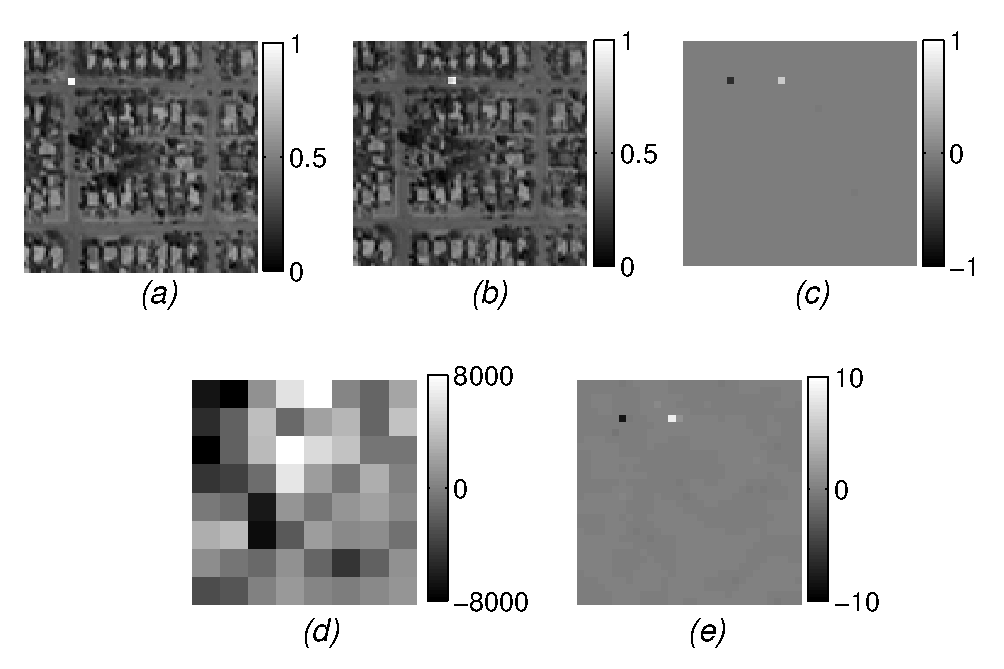
\includegraphics[scale=0.75]{scout_fig12_bg_un}
	\captionof{figure}[Difference frame 1 of a reconstruction video of two movers on a non-zero background.]{Difference frame 1 of a video demonstration of compressive tracking of a  $32 \times 32$ difference scene with a non-zero background. Scene background ©2012 Google. (a) ground- truth scene 1 (b) ground-truth scene 2 (c) ground-truth frame difference and (d) measured $8 \times 8$ frame difference, scaled so that it is discernible (e) reconstructed $32 \times 32$ difference frame}
	\label{fig:scout_fig12_bg_un}
\end{figure}


In the reconstruction of the ninth difference frame, the amplitude of one the movers had a lower amplitude, shown in \Cref{fig:scout_fig11_un}. Poor reconstruction tends to occur when two movers are located adjacent to each other in the ground-truth difference scene. This is an issue that can be traced to the system response matrix $\mb{H}$, locations next to each other have are more likely to have larger correlations in their respective \gls{psf}.


We also performed a more realistic experiment in which a mover simulates a vehicle driving on a street. This demonstrates that the \gls{scout} works well in situations with non-zero backgrounds. This sequence with the results for a single mover is also shown in Appendix \ref{app:scoutExpResults}. The first difference frame of this sequence is shown in \Cref{fig:scout_fig12_bg_un}. As seen in ground truth difference fram $\Delta \mb{f}$ shown in \Cref{fig:scout_fig12_bg_un}(c), the amplitude of the past and present mover locations in the ground-truth are lower than the zero background case. Therefore there is also less contrast in $\Delta \mb{g}$ the difference measurements in \Cref{fig:scout_fig12_bg_un}(d), which makes this case more sensitive to noise. 

The most notable feature in the non-zero background results is less quantitative agreement with the ground-truth, even when the calibration matrix is scaled according to \Cref{eq:ScoutCalibrationMatrixScaling}. There are several reasons for this: Nonlinearities in the overall system response that result from a nonlinear monitor “gamma” (mapping from pixel value to output brightness) and inter-pixel interactions that effect brightness. These effects are not captured during calibration as that is performed point-by-point (thus reducing inter-pixel effects) and with pixels that are fully-on or -off (thus avoiding effects from monitor gamma). Another possible reason is over-multiplexing, since the total light from each frame is increased, there is less dynamic range in the \gls{fpa}, and therefore detector non-linearity may be a source of error. Despite the lack of quantitative agreement, qualitative agreement is excellent and the movers are clearly identifiable agains the background in \Cref{fig:scout_fig12_bg_un}(e).



\section{Conclusion}

While the \gls{scout} architecture is well-suited for tracking applications, it does have limitations which make it less useful for general imaging applications. Without sparse scene motion, the priors used in reconstruction will lead to incorrect results. Reconstructions only show the locations of moving objects, and the sensing platform must be stationary relative to the scene so that frame differences are sparse. However, more sophisticated techniques could potentially estimate platform motion. Despite the limits of the \gls{scout}, the architecture is well-suited for applications such as fixed-camera wide-area surveillance where bandwidth, data volume, and cost are key concerns.

Many of the theoretical guarantees for \gls{compressive sensing} is not specialized or tuned for the block-circulant system matrix. As I mentioned in \Cref{chap:Formalism}, random coding has several theoretical properties that make them useful for compressive sensing. There has been some research work to investigate system matrices with Toeplitz and circulant structure \cite{bajwa2007toeplitz, rauhut2009circulant, romberg2009compressive}, however there has been relatively little work published discussing the approximately block-Toeplitz structure that naturally arises in optical systems such as \gls{scout} and theoretical guarantees like the ones force random coding. Two exceptions are \cite{sebert2008toeplitz, liu2008sparsesense}, which provide both theoretical evidence for the viability of CS system matrices with block-Toeplitz structure.


A completely parallel compressive imager would require as many encoding optical elements as simultaneous measurements. The \gls{scout} architecture eliminates this scaling issue by giving up the ability to implement arbitrary projections. Using a pair of masks at different distances to create a block-circulant system matrix, the system makes compressive measurements and reconstructs frame differences. The system can be optimized by adjusting system parameters such as mask pitch and defocus distance. Simulations demonstrated the use of the a modified coherence parameter as an efficient predictor of system matrix performance to optimize these parameters. An experimental system based on the \gls{scout} architecture successfully performed compressive motion tracking on scenes with zero and nonzero backgrounds in most instances. However, the reconstruction of difference scenes with adjacent mover locations caused issues due to the design or calibration of the system matrix. The system showed promising results using a general $\ell_1$-norm minimization algorithm and we believe that further research on sparse reconstruction with block-circulant system matrices may decrease reconstruction error. We also believe that non-isomorphic calibration techniques and adding further degrees of freedom in the design parameters could result in significant performance gains.




